\documentclass[10pt,twocolumn]{article}

\usepackage[utf8]{inputenc}
\usepackage[T1]{fontenc}
\usepackage{amsmath,amssymb}
\usepackage{graphicx}
\usepackage{booktabs}
\usepackage[colorlinks=false, pdfborder={0 0 0}]{hyperref}
\usepackage[margin=1in]{geometry}
\usepackage{xcolor}
\usepackage{microtype}
\usepackage[numbers,sort&compress]{natbib}
\usepackage{caption}
\usepackage{float}
\usepackage{stfloats}
\captionsetup{font=small,labelfont=bf}
\graphicspath{{figures/}}
\emergencystretch=3pt

\title{Local ancestry and IBD inference\\directly from pangenome based alignments}
\author{Franco L.\ Marsico$^1$, Silvia Buonaiuto$^1$, Laura Pignata$^1$, Farnaz Salehi$^1$,\\
Robert W.\ Williams$^1$, Pjotr Prins$^1$, Erik Garrison$^1$, Vincenza Colonna$^1$\\[0.5em]
{\normalsize $^1$Dept.\ of Genetics, Genomics and Informatics, UTHSC, USA}}
\date{}

\begin{document}

\maketitle

\textbf{Abstract.}
Traditional local ancestry and identity-by-descent (IBD) inference relies on variant
calls, introducing reference bias and requiring statistical phasing. Here we introduce
\texttt{$impop_k$}, a framework that infers local ancestry, IBS, IBD, and kinship
directly from pairwise sequence identity from haplotype-resolved pangenomes via hidden
Markov models. In simulations, ancestry concordance reaches 97.95\% (vs.\ 95.9\% for
RFMix) and IBD recall hits 96.9\% (vs.\ 90.6\% for hap-ibd); pedigree validation
yields 99.5\% founder painting concordance. Applied to human genomes (HPRCv2
assemblies, CEPH~1463), \texttt{$impop_k$} resolves American three-way admixture and
detects population-specific IBS enrichment at known selection targets, including the
lactase persistence locus. Across a bovine super-pangenome and inbred BXD mice, it
maps subspecies phylogeny and identifies founder ancestry tracts. Raw pangenomic based alignment similarity thus holds sufficient genealogical signal for robust whole-genome inference, bypassing variant catalogs, statistical phasing, and
population-specific reference panels.


\section{Introduction}

Two haplotypes that coalesce recently share long stretches of nearly identical sequence; the more remote the common ancestor, the more substitutions, indels, structural variants, and rearrangements accumulate. This relationship between coalescence time and sequence identity is the basis for both identity-by-descent (IBD) detection and local ancestry inference. Kingman's coalescent~\cite{kingman1982coalescent} provides the probabilistic framework: at a given locus, two lineages trace back to a common ancestor at a rate determined by the ancestral process, and expected pairwise divergence scales with that time under a neutral mutation model. Thompson unified pedigree-based and coalescent perspectives on IBD~\cite{thompson2013ibd}. Guo formalized the genomic consequence: the transmission of chromosomal segments through a pedigree follows a continuous-time Markov chain whose transition rates are governed by recombination~\cite{guo1994computation, guo1995proportion}, implying that windowed sequence identity tracks IBD status and ancestry as latent states along the genome. \texttt{$impop_k$} is built on this observation.

In practice, most widely used methods for IBD detection~\cite{browning2020hap_ibd, browning2013ibdseq, gusev2009germline, shemirani2021ilash, naseri2019rapid} and local ancestry inference~\cite{maples2013rfmix, browning2023flare} operate on phased VCF genotypes, introducing SNP ascertainment bias~\cite{lachance2012ascertainment}, excluding structural variation, and requiring statistical phasing whose errors concentrate at ancestry switch points~\cite{browning2023flare}. Graph-based approaches (PanGenie~\cite{ebler2022pangenie}, vg~\cite{garrison2018vg}) reduce ascertainment bias but remain tied to variants catalogued in a reference graph. ntRoot~\cite{ntroot2025} classifies ancestry from assemblies without alignment, but remains tied to a human-specific variant reference panel and outputs coarse superpopulation labels rather than genealogical tracts. Haplotype-resolved assemblies thus carry genealogical signal that current pipelines do not directly exploit.


 When two assemblies are aligned, the fraction of matching bases in consecutive genomic windows is a continuous readout of local relatedness. Assemblies for hundreds of individuals are now available through the Human Pangenome Reference Consortium (HPRC)~\cite{liao2023hprc}. Windowed pairwise identity can be computed from such alignments using tools such as \texttt{impg}~\cite{impg}. Although the identity contrast between genomic states is subtle, its consistency across consecutive windows
matches exactly the structure Guo's model predicts~\cite{guo1994computation, guo1995proportion}. \texttt{$impop_k$} takes this windowed pairwise identity as input, from pangenome alignments, graph-based approaches, or other sources, and recovers IBS, IBD and ancestry tracts.

Here we evaluate \texttt{$impop_k$} (Fig.~\ref{fig:overview}) on simulations built from real HPRC assemblies, on the CEPH~1463 platinum pedigree, and on non-human models such as the bovine super-pangenome and BxD mice line.

\begin{figure*}[t]
\centering
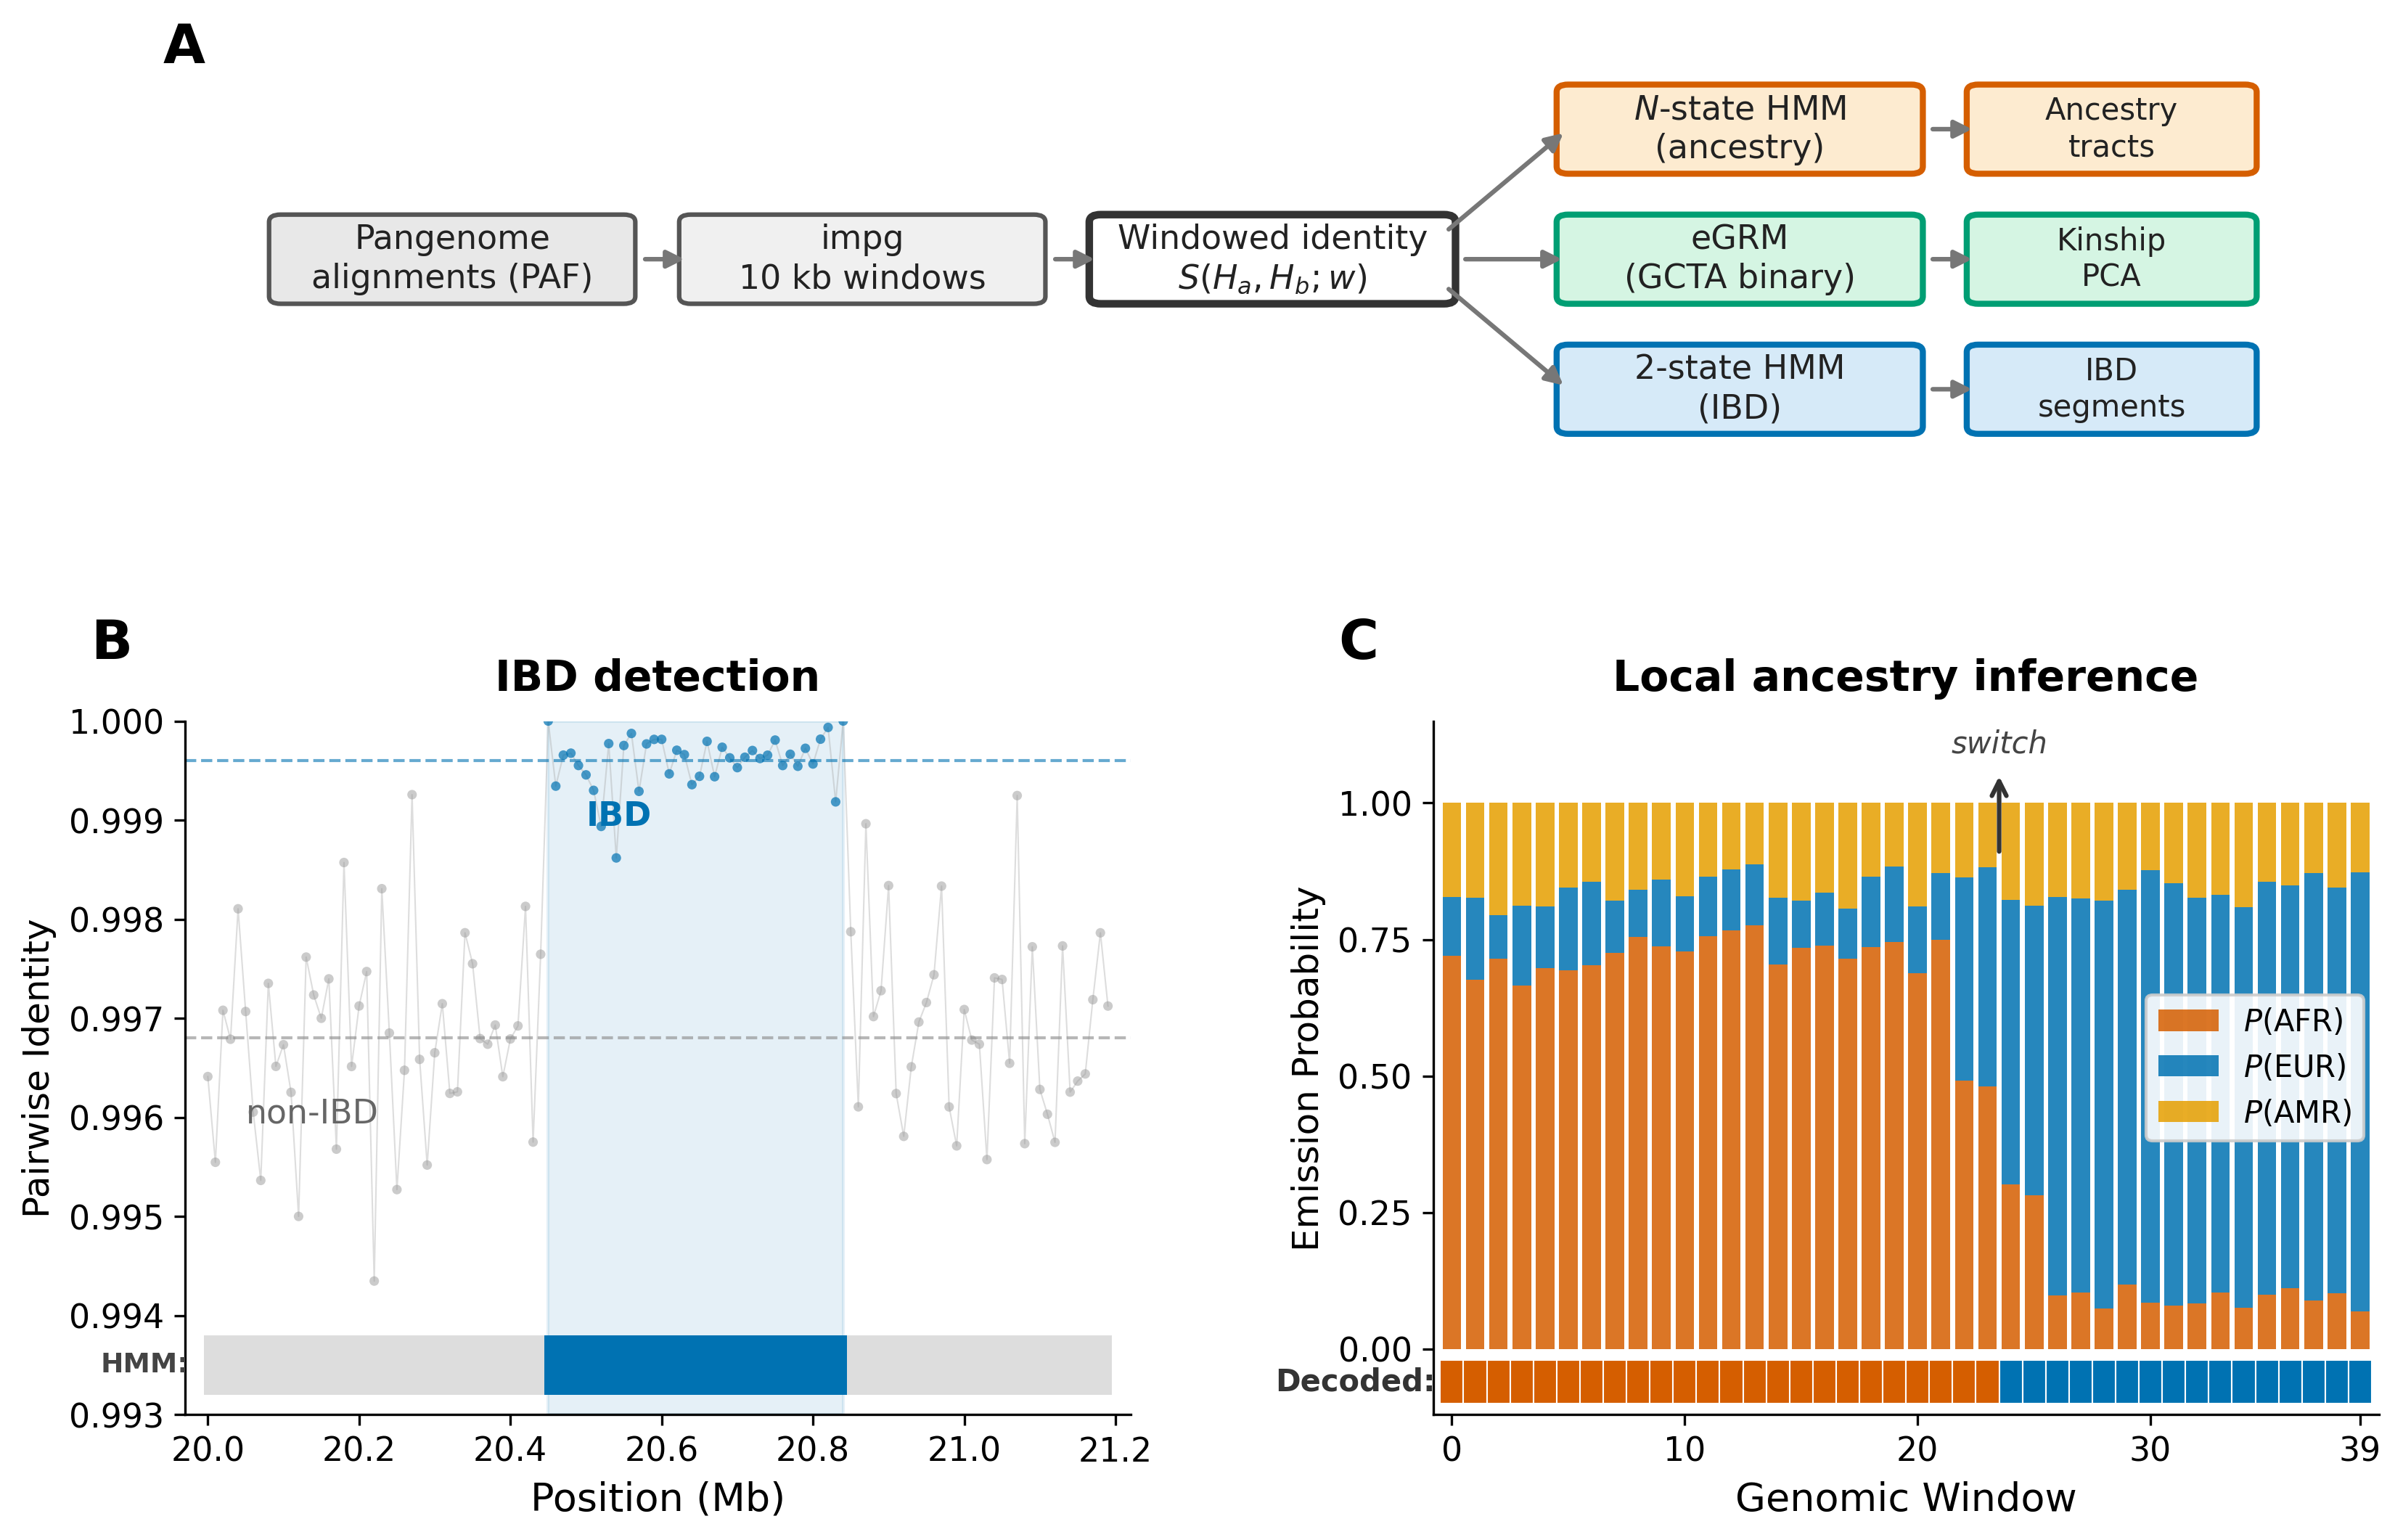
\includegraphics[width=0.8\textwidth]{fig0_method_overview.png}
\caption{\texttt{$impop_k$} overview. \textbf{A)}~Pangenome alignments are converted by \texttt{impg} into a windowed identity matrix, which feeds a 2-state IBD HMM or an $N$-state ancestry HMM. \textbf{B)}~IBD windows show elevated identity ($\Delta\approx 0.003$). \textbf{C)}~Per-population identity tracks are compared with adaptive temperatures; the decoded ancestry is shown at the bottom.}
\label{fig:overview}
\end{figure*}


% ──────────────────────────────────────────────────────────────
\section{Methods}

\textbf{Pairwise identity from pangenome alignments.}
Given a set of haplotype-resolved assemblies, their all-to-reference alignments, and a reference coordinate system, we partition each chromosome into non-overlapping windows of size $w$ (10 kb throughout). For haplotypes $H_a, H_b$ at window $t$, we denote by $S(H_a, H_b; t)$ the pairwise sequence identity in that window. Several approaches and metrics can be used to compute $S$. In the examples presented in this work, we used the estimated identity reported by \texttt{impg}~\cite{impg}, using the Jaccard index of the aligned positions of the two haplotypes within the window.

  \textbf{Identity-by-state (IBS).}
  A window is classified as IBS between two haplotypes when $S(H_a, H_b; t) \geq \theta$ for a user-defined threshold $\theta$. The fraction of IBS windows within a genomic region provides a measure of local haplotype sharing that can be compared across populations to detect signals of selection or demographic history.


\textbf{IBD detection (2-state HMM).}
 We model IBD with a 2-state HMM and Gaussian emissions (Fig.~\ref{fig:overview}B). Emission parameters are initialized from population-specific nucleotide diversity priors when available and then re-estimated from the observed identity distribution via k-means clustering and Baum-Welch expectation-maximization~\cite{baum1970maximization}. This makes the model species and population versatile. Transition probabilities encode expected segment length and optionally scale with genetic distance. Segments are decoded via Viterbi and filtered by length and LOD score.

  \textbf{Kinship estimation.}
For a diploid pair $(A, B)$, the kinship coefficient is estimated as $$\hat{\theta} = \sum_{\alpha,\beta} L_{\text{IBD}}(A_\alpha, B_\beta)\, /\, 4L$$, where $L_{\text{IBD}}$ is the total detected IBD length for each of the four haplotype pairings and $L$ is the chromosome length~\cite{thompson2013ibd}.

\textbf{Ancestry inference ($N$-state HMM).}
For a query haplotype $q$ and $K$ reference populations, the emission at window $t$ for population $k$ is $f_k(t) = \max_{h \in \mathcal{H}_k} S(q, h; t)$, the highest identity to any haplotype in that population. Log-emissions follow a softmax:
$$\log P(o_t \mid s_t{=}k) = \frac{f_k(t)}{\tau} - \log \sum_{j=1}^{K}
\exp\!\left(\frac{f_j(t)}{\tau}\right)  $$
 We used per-pair adaptive temperatures through Bradley-Terry pairwise comparison model: $P_{ij}(i;t) = \sigma\bigl((f_i{-}f_j)/\tau_{ij}\bigr)$, with $\tau_{ij}$ estimated from the empirical distribution of $|f_i(t){-}f_j(t)|$ across windows (Fig.~\ref{fig:overview}C).

\textbf{Structurally variable regions and support-weighted emissions.}
Pangenome depth ($d_t = $ number of haplotypes that align in window $t$, normalized by panel size) flags windows where part of the reference panel does not align to the reference coordinate system, typically due to insertions, large indels, or other structural haplotypes absent from the linear reference. We compute $d_t$ directly from the alignment with \texttt{impg depth}~\cite{impg}. Optionally, the ancestry HMM accepts a per-window weight $w_t = d_t / \max_t d_t \in [0, 1]$ and the log-emission row is shrunk toward a uniform distribution: $\log P'(o_t \mid s_t) = w_t \log P(o_t \mid s_t) + (1 - w_t) \log(1/K)$. When $w_t \to 0$ — a centromeric or low-coverage window — the local emission carries no information and the posterior is determined by the flanking windows through the transition prior, instead of by an unreliable identity measurement on a degraded alignment. The HMM is otherwise unchanged. This is exposed as the \texttt{-{}-window-weights} option of the \texttt{ancestry} binary.

\textbf{Simulations.}
Admixed or related haplotypes were constructed by stitching real HPRC assembly segments along msprime-generated tracts~\cite{kelleher2016msprime}, preserving the sequence characteristics of the source pangenome. For ancestry, 10 haplotypes with known admixture (70\% AFR, 30\% EUR on chr12, 133\,Mb) were evaluated against a 46-haplotype reference panel with donor exclusion, alongside matched RFMix on phased VCFs from the same sequences. For IBD, 100 diploid individuals (14 with known pedigree relationships from full siblings through third cousins, plus 86 unrelated controls) were simulated on chr12:0--50\,Mb ($N_e{=}10{,}000$) using the msprime pedigree model. Ground-truth IBD segments were extracted from the tree sequences; hap-ibd was run on phased VCFs from the same individuals.

\textbf{Performance metrics} Ancestry concordance is the fraction of windows where the decoded population label matches the ground truth. IBD recall is the fraction of ground-truth pairs sharing above a length threshold that are also detected by the method.


% ──────────────────────────────────────────────────────────────
\section{Results}


\subsection{Simulation-based evaluation}

We evaluated ancestry and IBD on controlled simulations where the ground truth is known exactly, comparing it against matched VCF-based methods.

\subsubsection{Ancestry}
\label{sec:sim_ancestry}

Aggregating across all simulated haplotypes, impop with automatically estimated parameters reached 96.5\% concordance, above RFMix's 95.9\% on the same panel (Table 1). With optimized inference parameters, concordance reached 97.95\%.


\begin{table}[H]
\centering
\caption{Ancestry concordance using simulated haplotypes, 133\,Mb each, 46-haplotype panel.}
\label{tab:sim_ancestry}
\small
\begin{tabular}{@{}lccc@{}}
\toprule
\textbf{Configuration} & \textbf{Conc.} & $\mathbf{F1_{\textsc{afr}}}$ & $\mathbf{F1_{\textsc{eur}}}$ \\
\midrule
RFMix                     & 95.9\%           & 0.953          & 0.942          \\
\texttt{$impop_k$} (auto)      & 96.5\%           & 0.969          & 0.960          \\
\texttt{$impop_k$} (optimized) & \textbf{97.95\%} & \textbf{0.982} & \textbf{0.977} \\
\bottomrule
\end{tabular}
\end{table}


Per-haplotype analysis of the optimized configuration shows \texttt{$impop_k$} achieving higher concordance than RFMix on 7 of 10 haplotypes (Fig.~\ref{fig:sim_ancestry}B), with the largest margin at 17.0 percentage points on a haplotype where RFMix drops to 81.4\%. In the remaining three, RFMix leads by 3.2, 0.9, and 0.1 percentage points. Errors concentrate at switch boundaries and in short tracts. Confusion matrices (Fig.~\ref{fig:sim_ancestry}E) show that RFMix over-calls EUR at boundaries at 2.88$\times$ the reverse rate, while the optimized \texttt{$impop_k$} configuration reduces this asymmetry to 1.19$\times$.

\begin{figure*}[t]
\centering
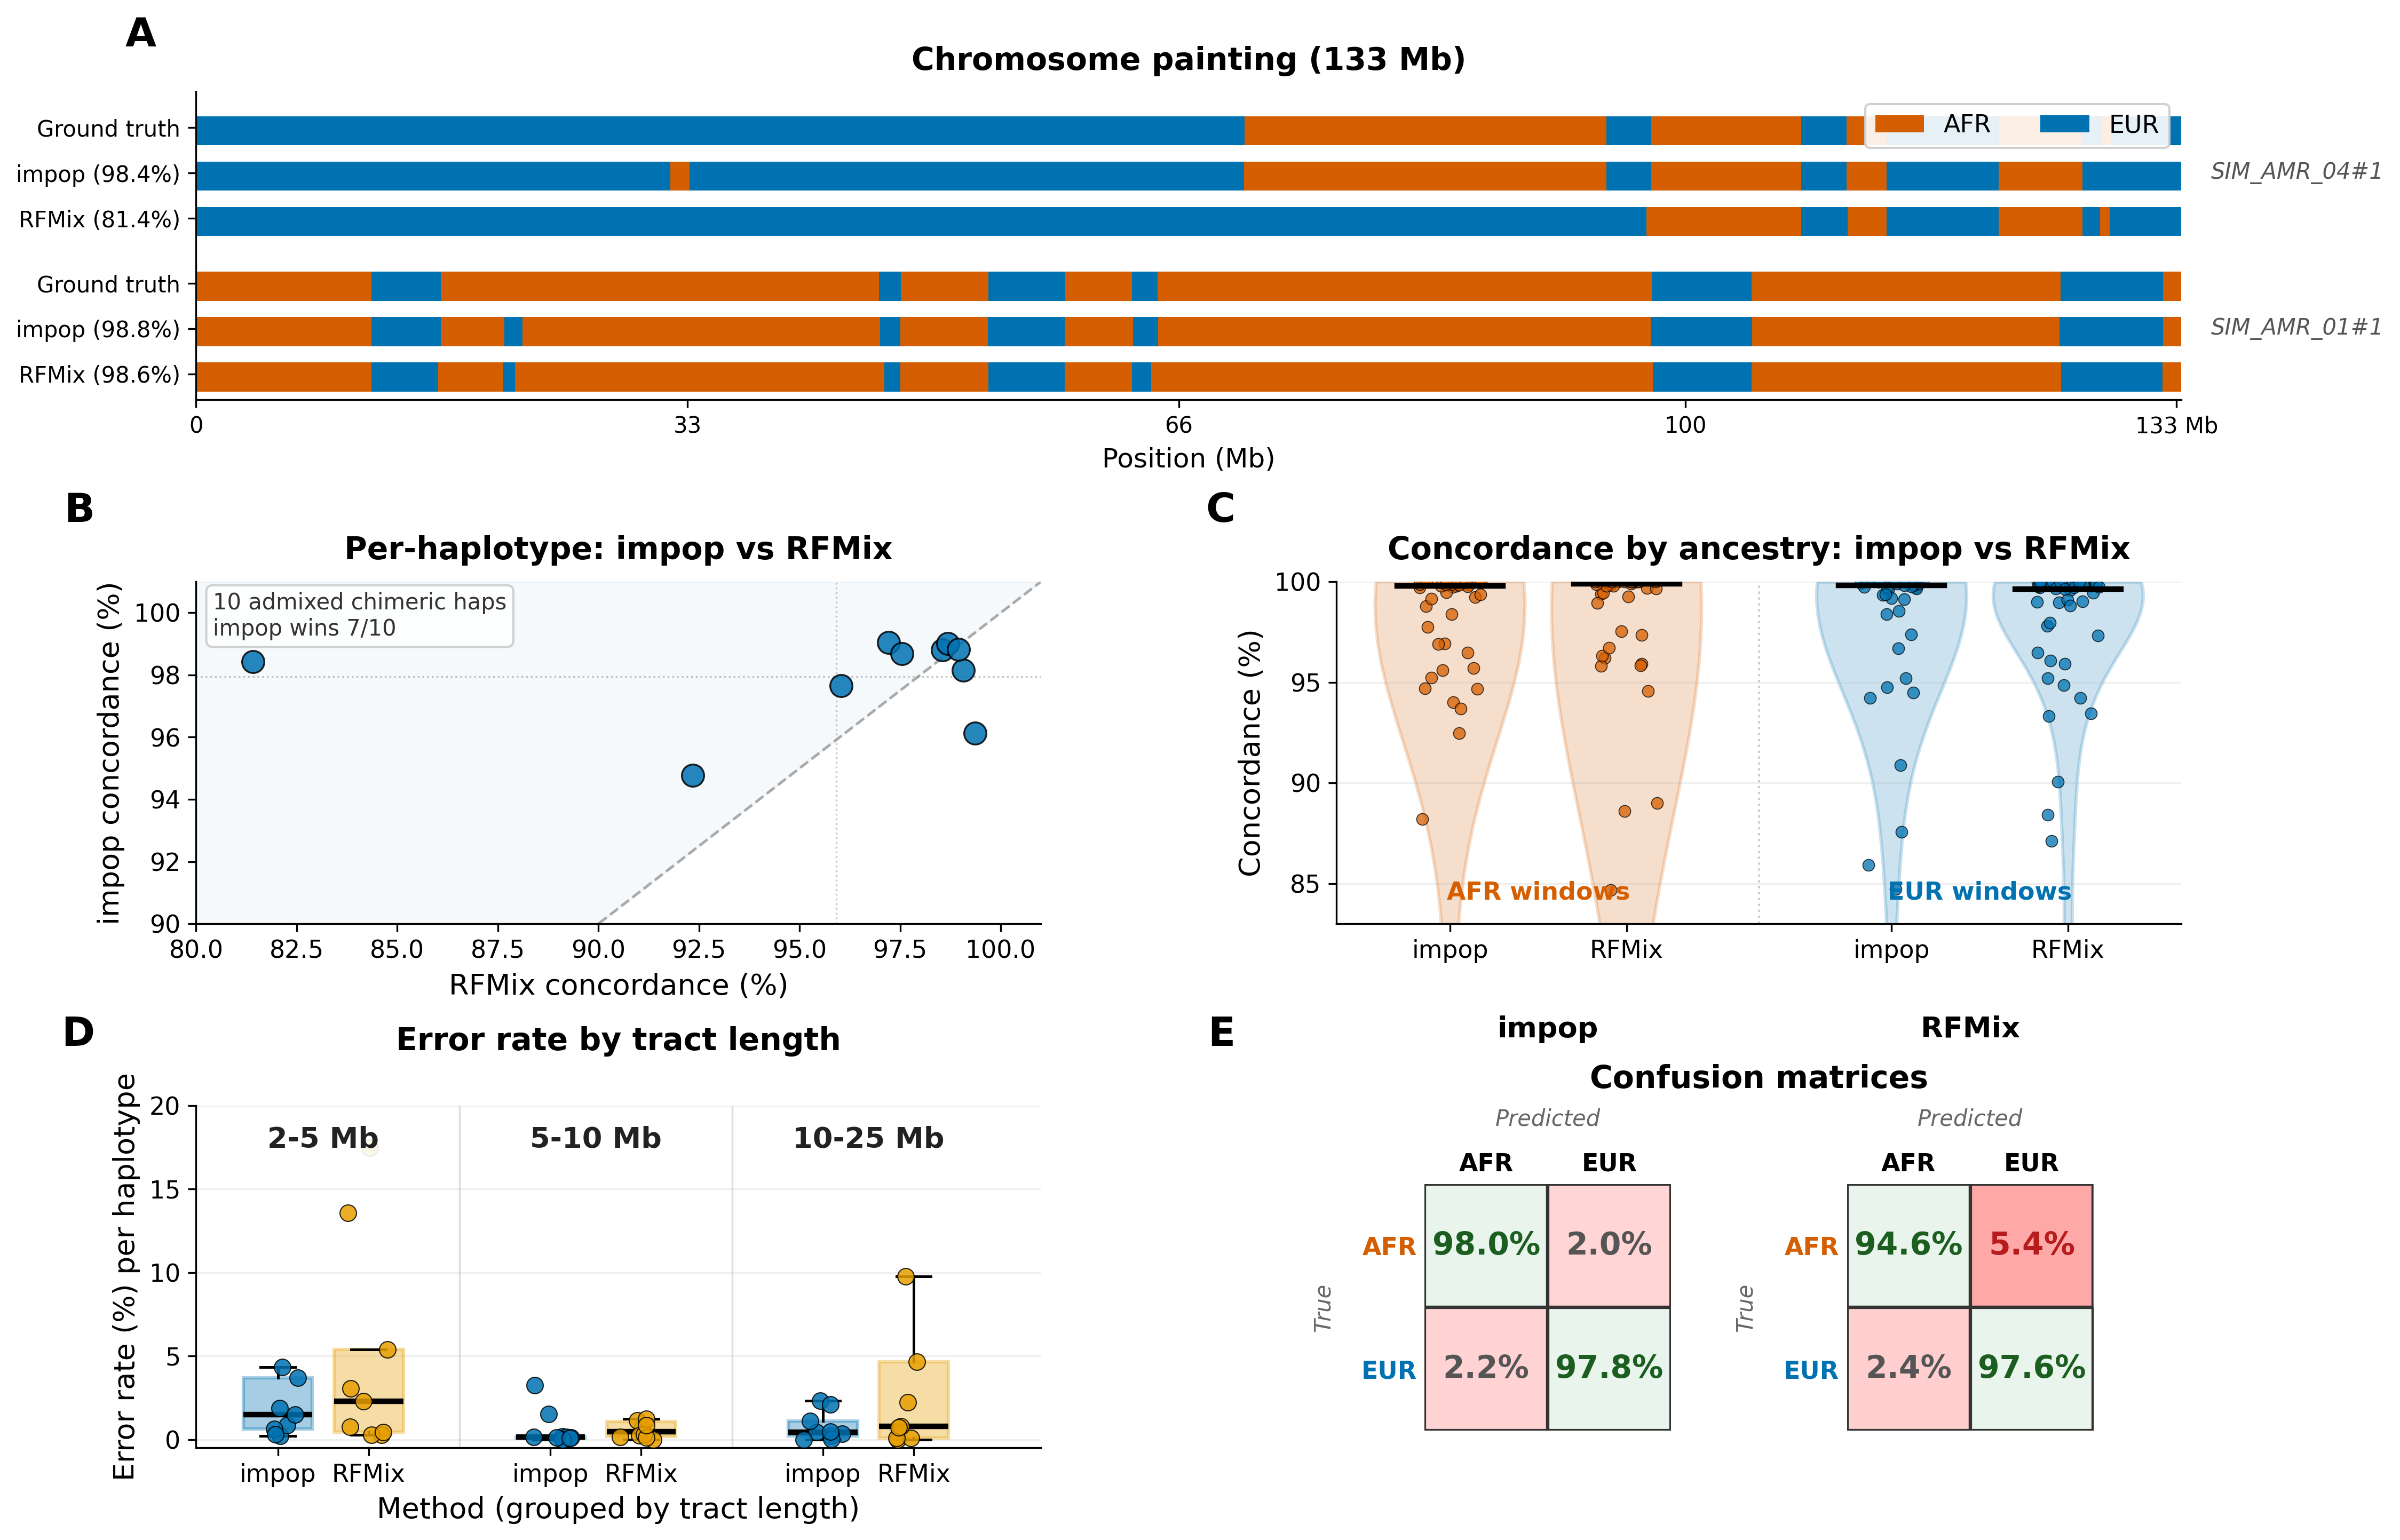
\includegraphics[width=0.85\textwidth]{fig1_simulation_4panel.png}
\caption{Ancestry validation (chr12, 133\,Mb). \textbf{A)}~Chromosome painting: ground truth, \texttt{$impop_k$}, RFMix. \textbf{B)}~Per-haplotype concordance (7/10 above diagonal). \textbf{C)}~Concordance by ancestry. \textbf{D)}~Error rate by tract length. \textbf{E)}~Confusion matrices.}
\label{fig:sim_ancestry}
\end{figure*}

\subsubsection{Identity-by-descent}
\label{sec:sim_ibd}

Of 32 ground-truth IBD pairs with segments $\geq$1.5\,Mb, \texttt{$impop_k$} identifies 31 (recall 96.9\%) and hap-ibd identifies 29 (90.6\%). The gap is concentrated among distant relatives, where \texttt{$impop_k$} detects 27 of 28 pairs and hap-ibd 25; at the $\geq$2\,Mb threshold both methods converge to 95.7\%. hap-ibd achieves finer boundary precision, reflecting its SNP-level resolution. Summing detected IBD across the four haplotype pairings per diploid pair yields a kinship estimate that tracks expected pedigree values with Pearson $r = 0.975$ across 76 pairs sharing any detectable IBD (Fig.~\ref{fig:ibd_sim}C). Full siblings are placed at $\hat{\theta} = 0.28$.

\begin{figure*}[t]
\centering
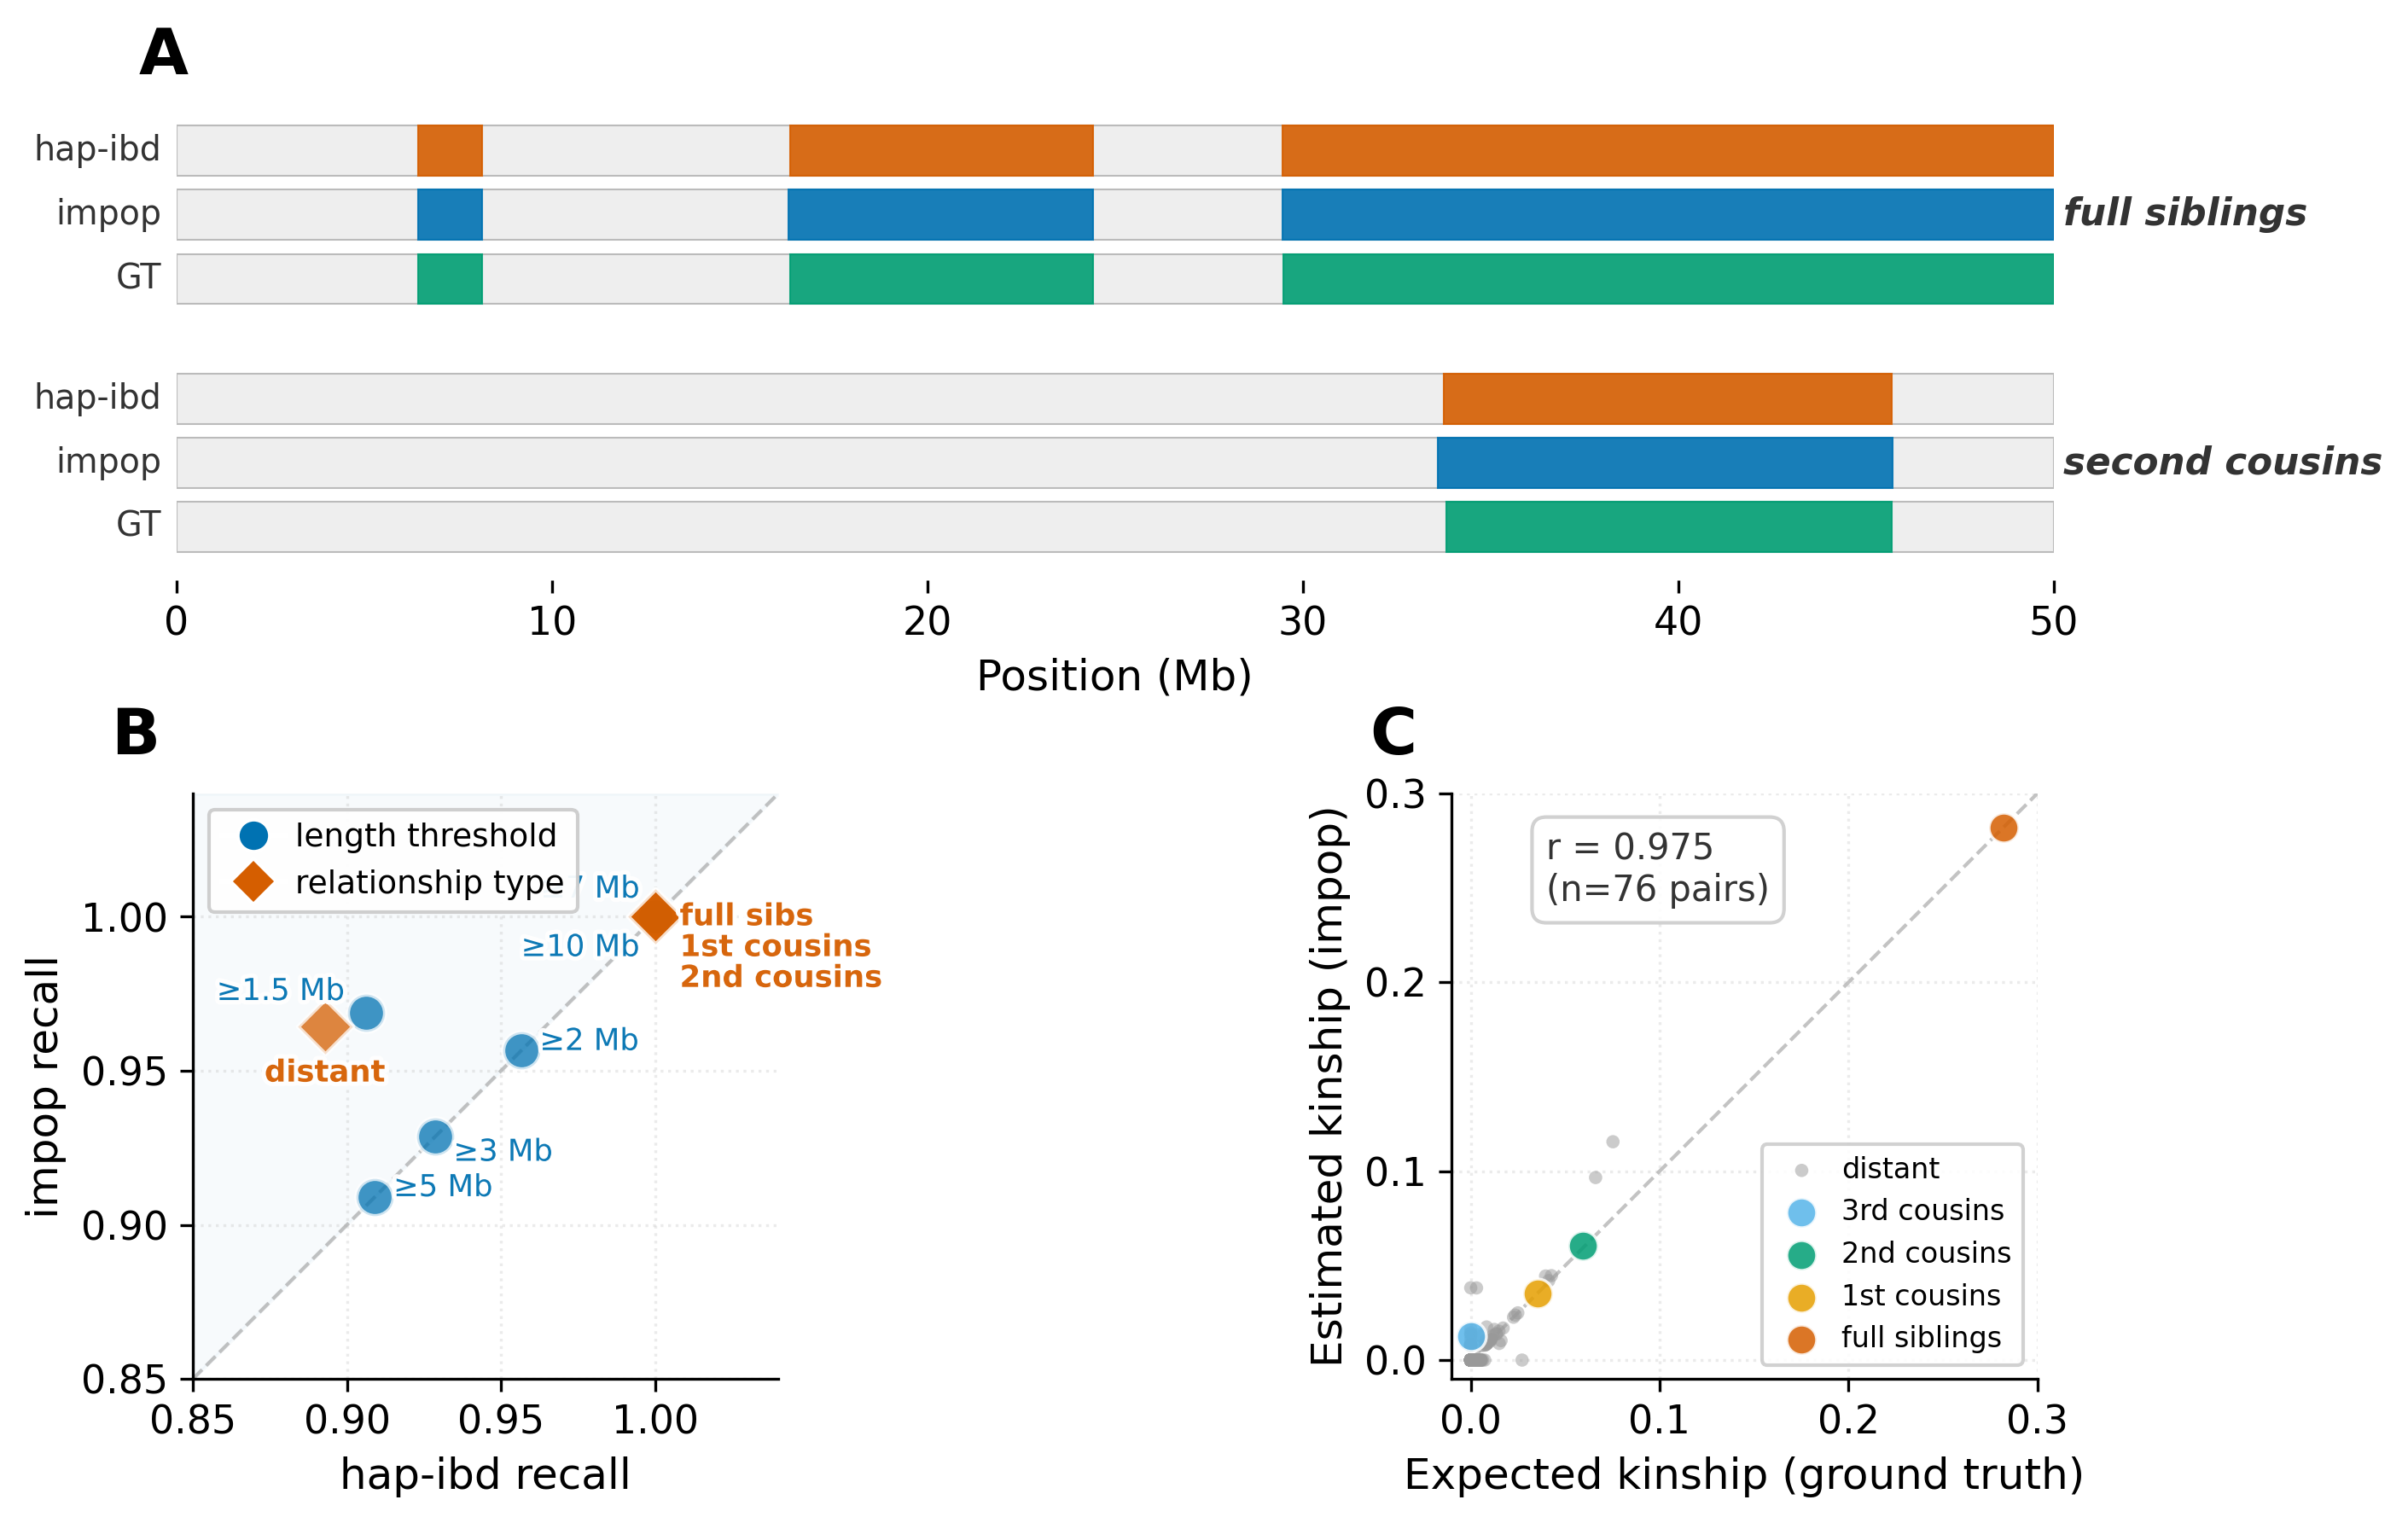
\includegraphics[width=0.85\textwidth]{fig3_ibd_simulation.png}
\caption{IBD detection (chr12:0--50\,Mb). \textbf{A)}~Chromosome painting of two pedigree pairs. \textbf{B)}~Method agreement across 10 conditions. \textbf{C)}~Kinship from detected IBD ($r=0.975$, $n=76$ pairs).}
\label{fig:ibd_sim}
\end{figure*}

\subsection{Real data}

\subsubsection{CEPH 1463 founder painting}
\label{sec:platinum}

The CEPH~1463 three-generation pedigree (Fig.~\ref{fig:platinum}A) provides biological ground truth independent of simulation. Four grandparents segregate their haplotypes through two parents into five grandchildren. Ground truth inheritance vectors, specifying which grandparent each segment comes from, were computed from HiFi-based DeepVariant calls using the \texttt{Platinum-Pedigree-Inheritance} toolkit~\cite{platinum_ped}.

With the HMM configured for four states (one per grandparent), concordance on chr1 averaged 99.5\% across 10 haplotypes (range: 99.1--100.0\%; Fig.~\ref{fig:platinum}C). The painting closely matches the ground truth (Fig.~\ref{fig:platinum}B). Highest uncertainty occurs at switch boundaries and in the centromeric region, where alignments are sparse. The high concordance reflects the identity contrast between unrelated founders ($\Delta \approx 0.003$), which, although comparable in magnitude to the population-level ancestry signal, benefits from a simpler four-state discrimination problem with longer tracts.

\begin{figure*}[t]
\centering
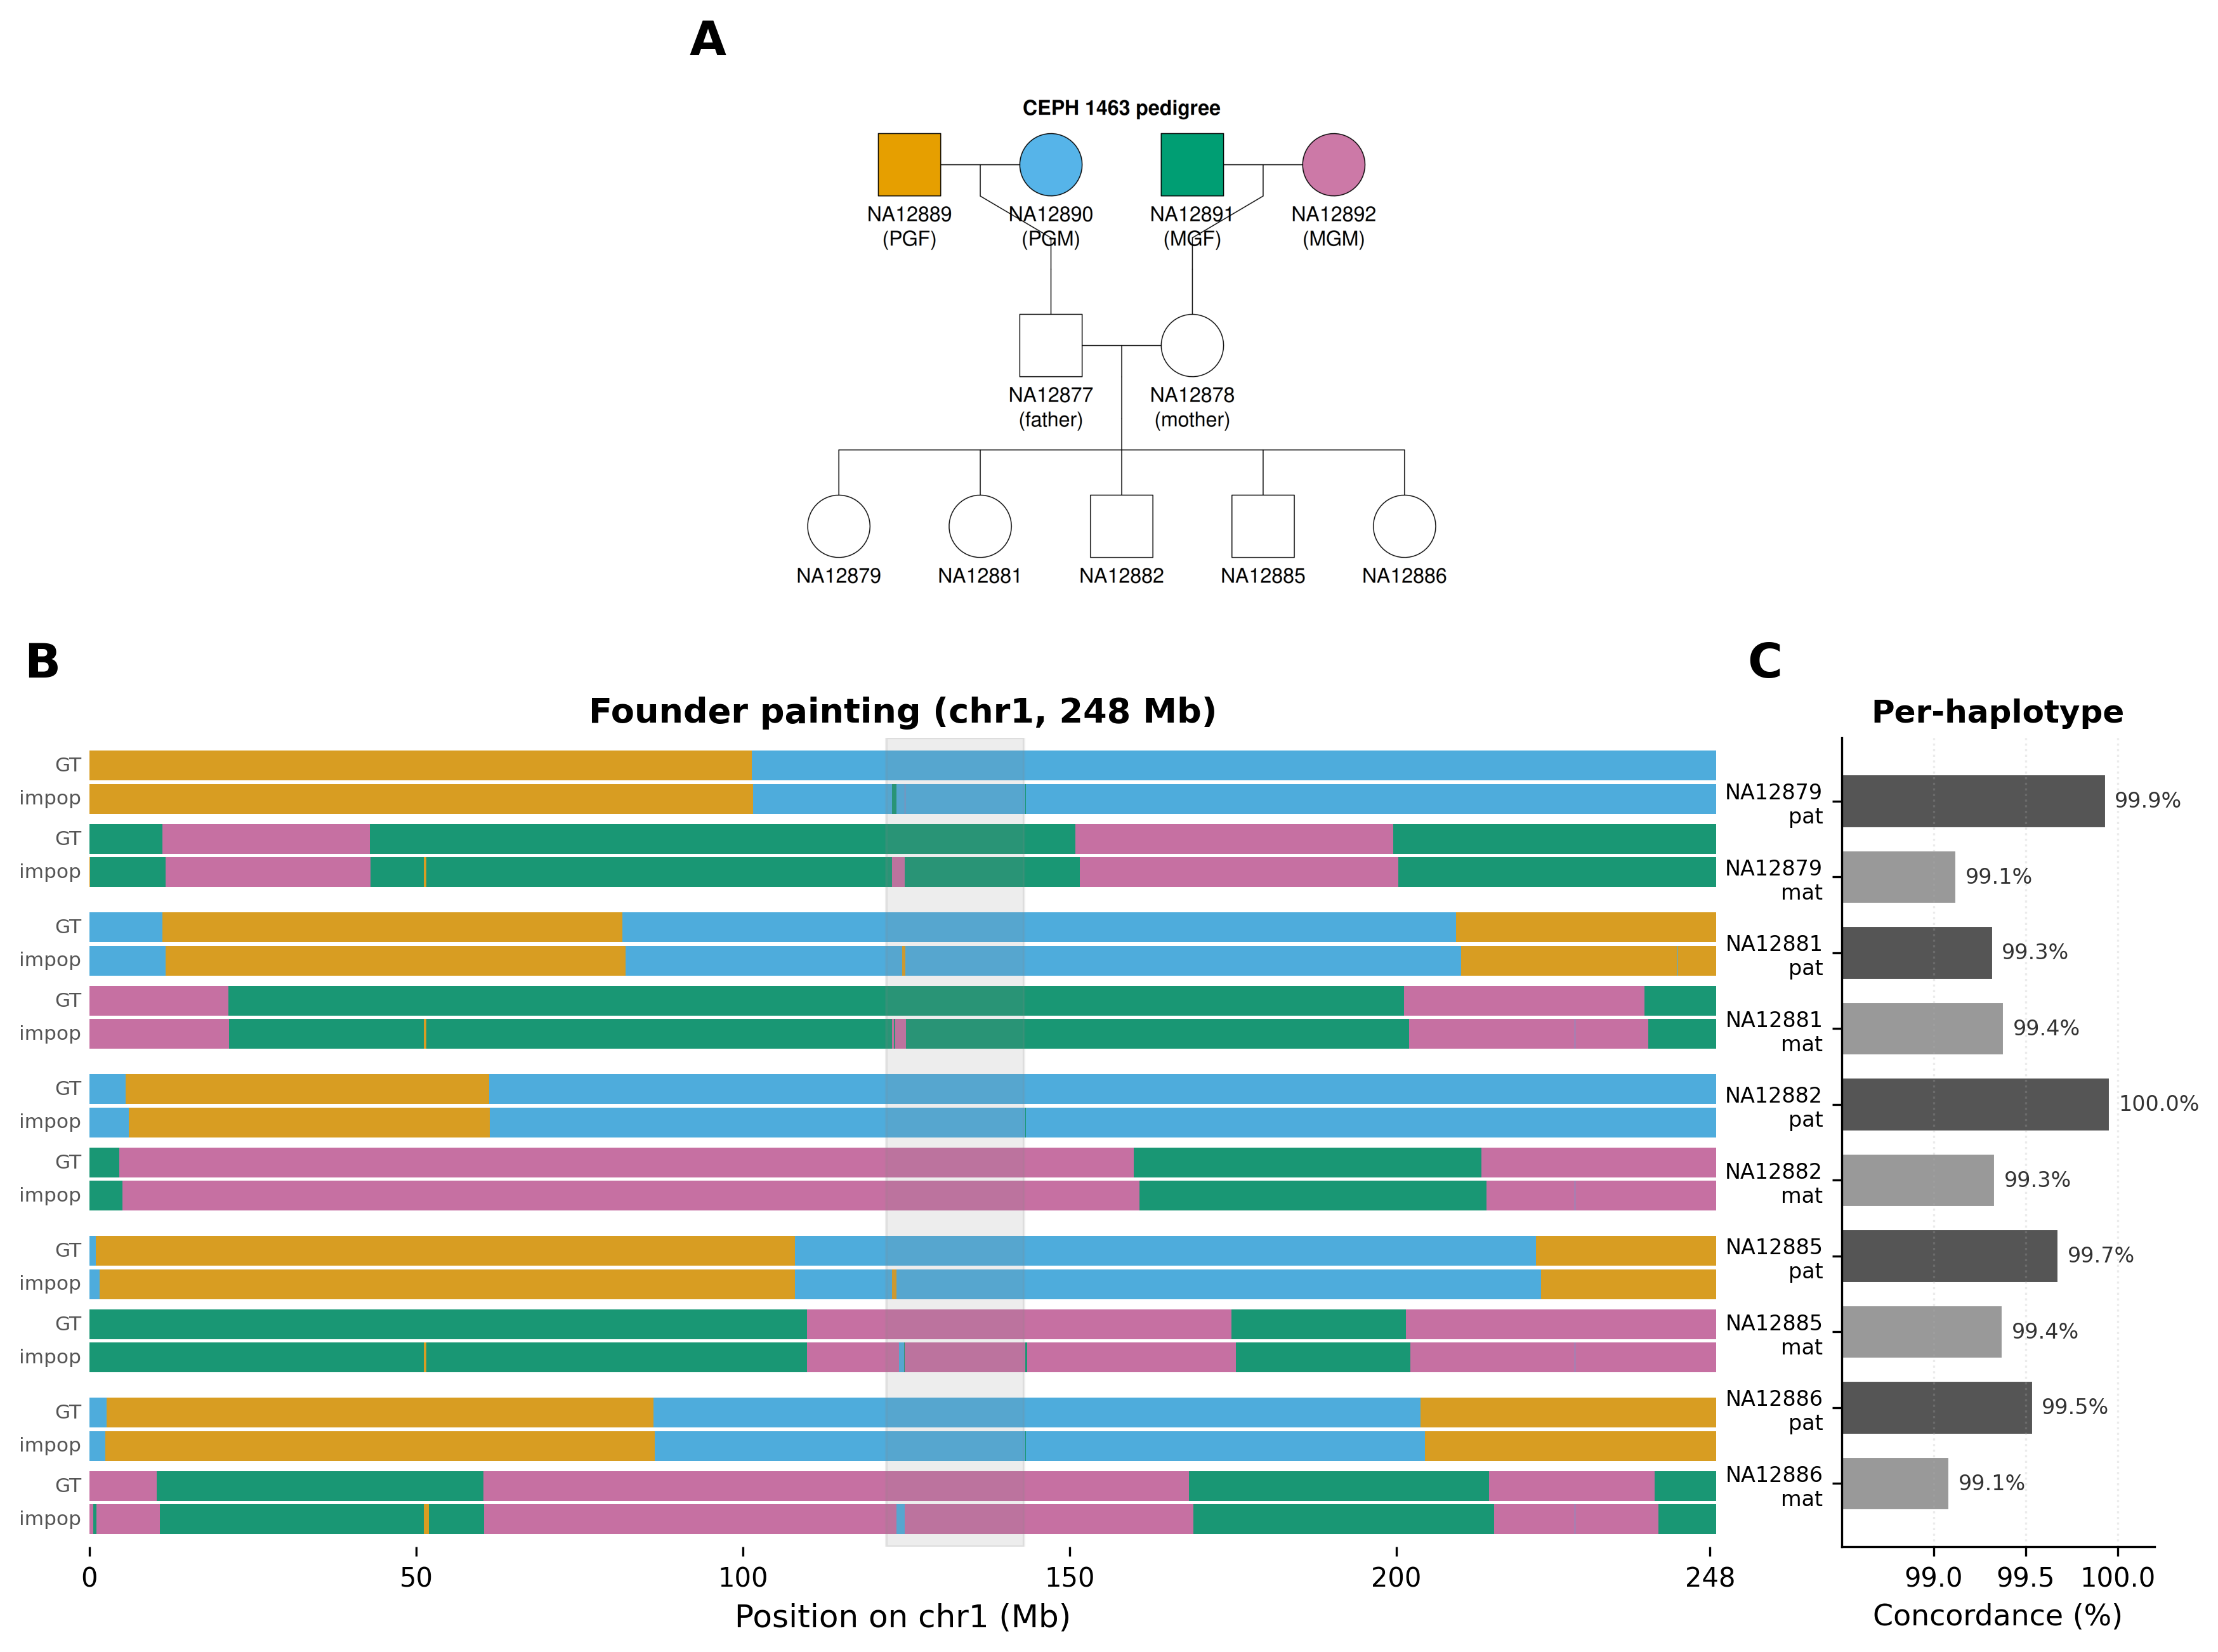
\includegraphics[width=0.85\textwidth]{fig4_platinum_pedigree.png}
\caption{CEPH~1463 founder painting (chr1, 248\,Mb). \textbf{A)}~Three-generation pedigree. \textbf{B)}~Paired tracks: ground truth (top) and \texttt{$impop_k$} (bottom). \textbf{C)}~Per-haplotype concordance (segments $\geq$10\,Mb; range 99.1--100.0\%).}
\label{fig:platinum}
\end{figure*}

  \subsubsection{Three-way admixture and natural selection in HPRC}
  \label{sec:hprc_real}

  As an exploratory analysis, we inferred three-way local ancestry (AFR, EUR, AMR) on chr1 (248\,Mb) for five admixed American individuals from the HPRC panel. Figure~\ref{fig:hprc_real}A shows the chromosome painting for one of those haplotypes. It carries large AMR tracts with interspersed EUR and AFR segments. This three-way characteristic is also confirmed with RFmixv2 and is well-documented in the Americas.

  \begin{figure}[ht]
  \centering
  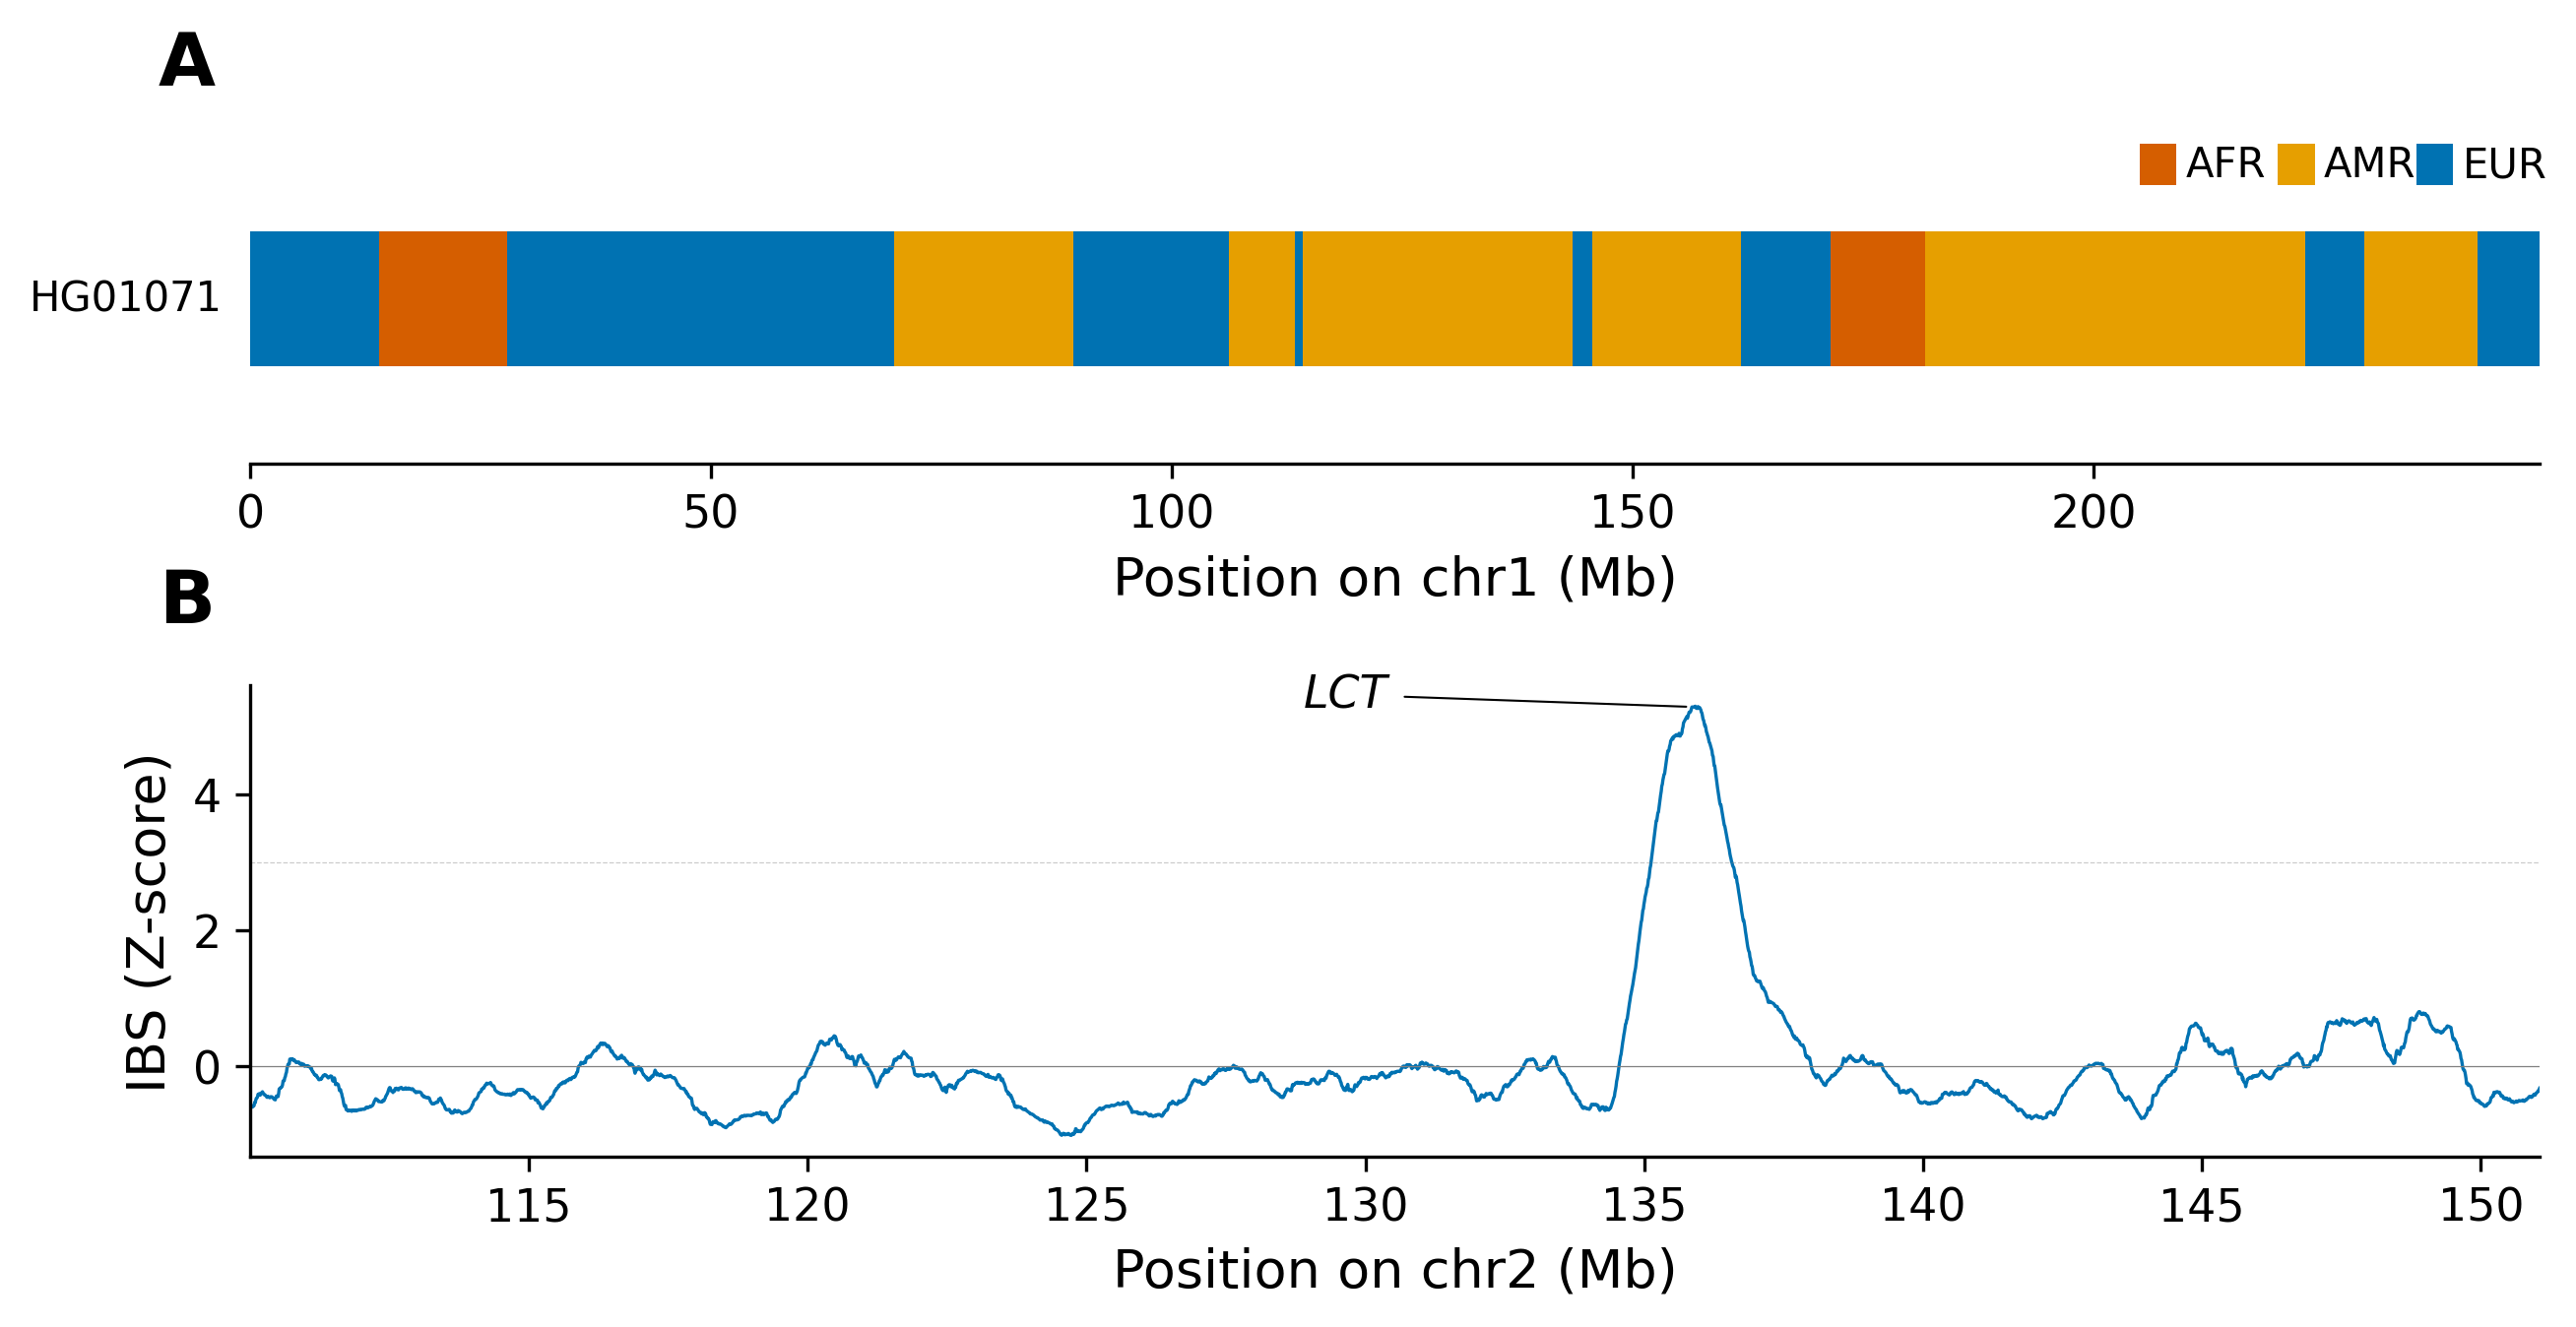
\includegraphics[width=0.5\textwidth]{fig_hprc_real.png}
  \caption{HPRC real data. \textbf{A)}~Three-way local ancestry on chr1
  for two Puerto Rican individuals. \textbf{B)}~EUR IBS sharing Z-score on
  chr2; the lactase persistence locus \emph{LCT} peaks at 5.3\,SD.}
  \label{fig:hprc_real}
  \end{figure}


  The same windowed identity data used for IBD and ancestry deconvolution can be scanned for regions of elevated within-population haplotype sharing, defining identity-by-state (IBS). On chr2, 25 HPRC individuals, we computed the fraction of within-population EUR haplotype pairs with identity exceeding 0.9999 and smoothed over 1\,Mb windows. The lactase persistence locus \emph{LCT} ($\sim$136\,Mb) produces a peak of 5.3 standard deviations above the EUR genome-wide mean (Fig.~\ref{fig:hprc_real}B), consistent with the well-documented European selective sweep at this locus~\cite{bersaglieri2004lct}.

\subsubsection{Structural-haplotype-aware ancestry at the TAS2R cluster}
\label{sec:tas2r_bubble}

A second class of advantage is visible at regions where the linear reference itself misses ancestry-informative variation. The chr12 TAS2R bitter-receptor cluster harbours a $\sim$4.5\,kb insertion enriched in West African genomes that is absent from both GRCh38 and the T2T-CHM13 reference. We detected this insertion directly from the pangenome alignment using \texttt{impg depth}: at chr12:10{,}952{,}775--10{,}957{,}250, only 218 of the 234 HPRCv2 + GRCh38 haplotypes align (16 missing), and all 15 non-reference missing haplotypes belong to African populations, giving a frequency of $\sim$12\% in HPRC AFR samples and 0\% elsewhere (Fig.~\ref{fig:tas2r}A). One HPRCv2 individual, HG01960 (1000G ACB), carries this African-specific structural haplotype.

We built 50 admixed chimeras (70\% AFR / 30\% EUR, $\sim$10 generations) using a 46-haplotype donor-excluded reference panel and used the 10 chimeras built from HG01960 as the AFR donor as a controlled test set; of those, 9 have AFR ground truth at the TAS2R core and 1 has EUR ground truth (CHIM\_38). The locus carries no biallelic SNPs callable from the chimeras' read-mapping, so FLARE has fewer than two variants per 10\,kb window inside the bubble (Fig.~\ref{fig:tas2r}B), and RFMix interpolates from flanking SNPs whose identity profile favours EUR (Fig.~\ref{fig:tas2r}C). Restricted to the 9 AFR-ground-truth chimeras at the 30\,kb core, RFMix calls AFR correctly in 0/9 cases, FLARE in 0/9, and \texttt{$impop_k$} with uniform 10\,kb windows in 1/9. With windows partitioned at the bubble boundaries and \texttt{-{}-window-weights} active, \texttt{$impop_k$} calls AFR correctly in 9/9 (Fig.~\ref{fig:tas2r}D). Two of these three failures (RFMix, uniform-window \texttt{$impop_k$}) are recovered without changing the algorithm: only the windowing and the per-window weights change, exposing pangenome signal that is invisible to any SNP-based method.

\begin{figure}[ht]
\centering
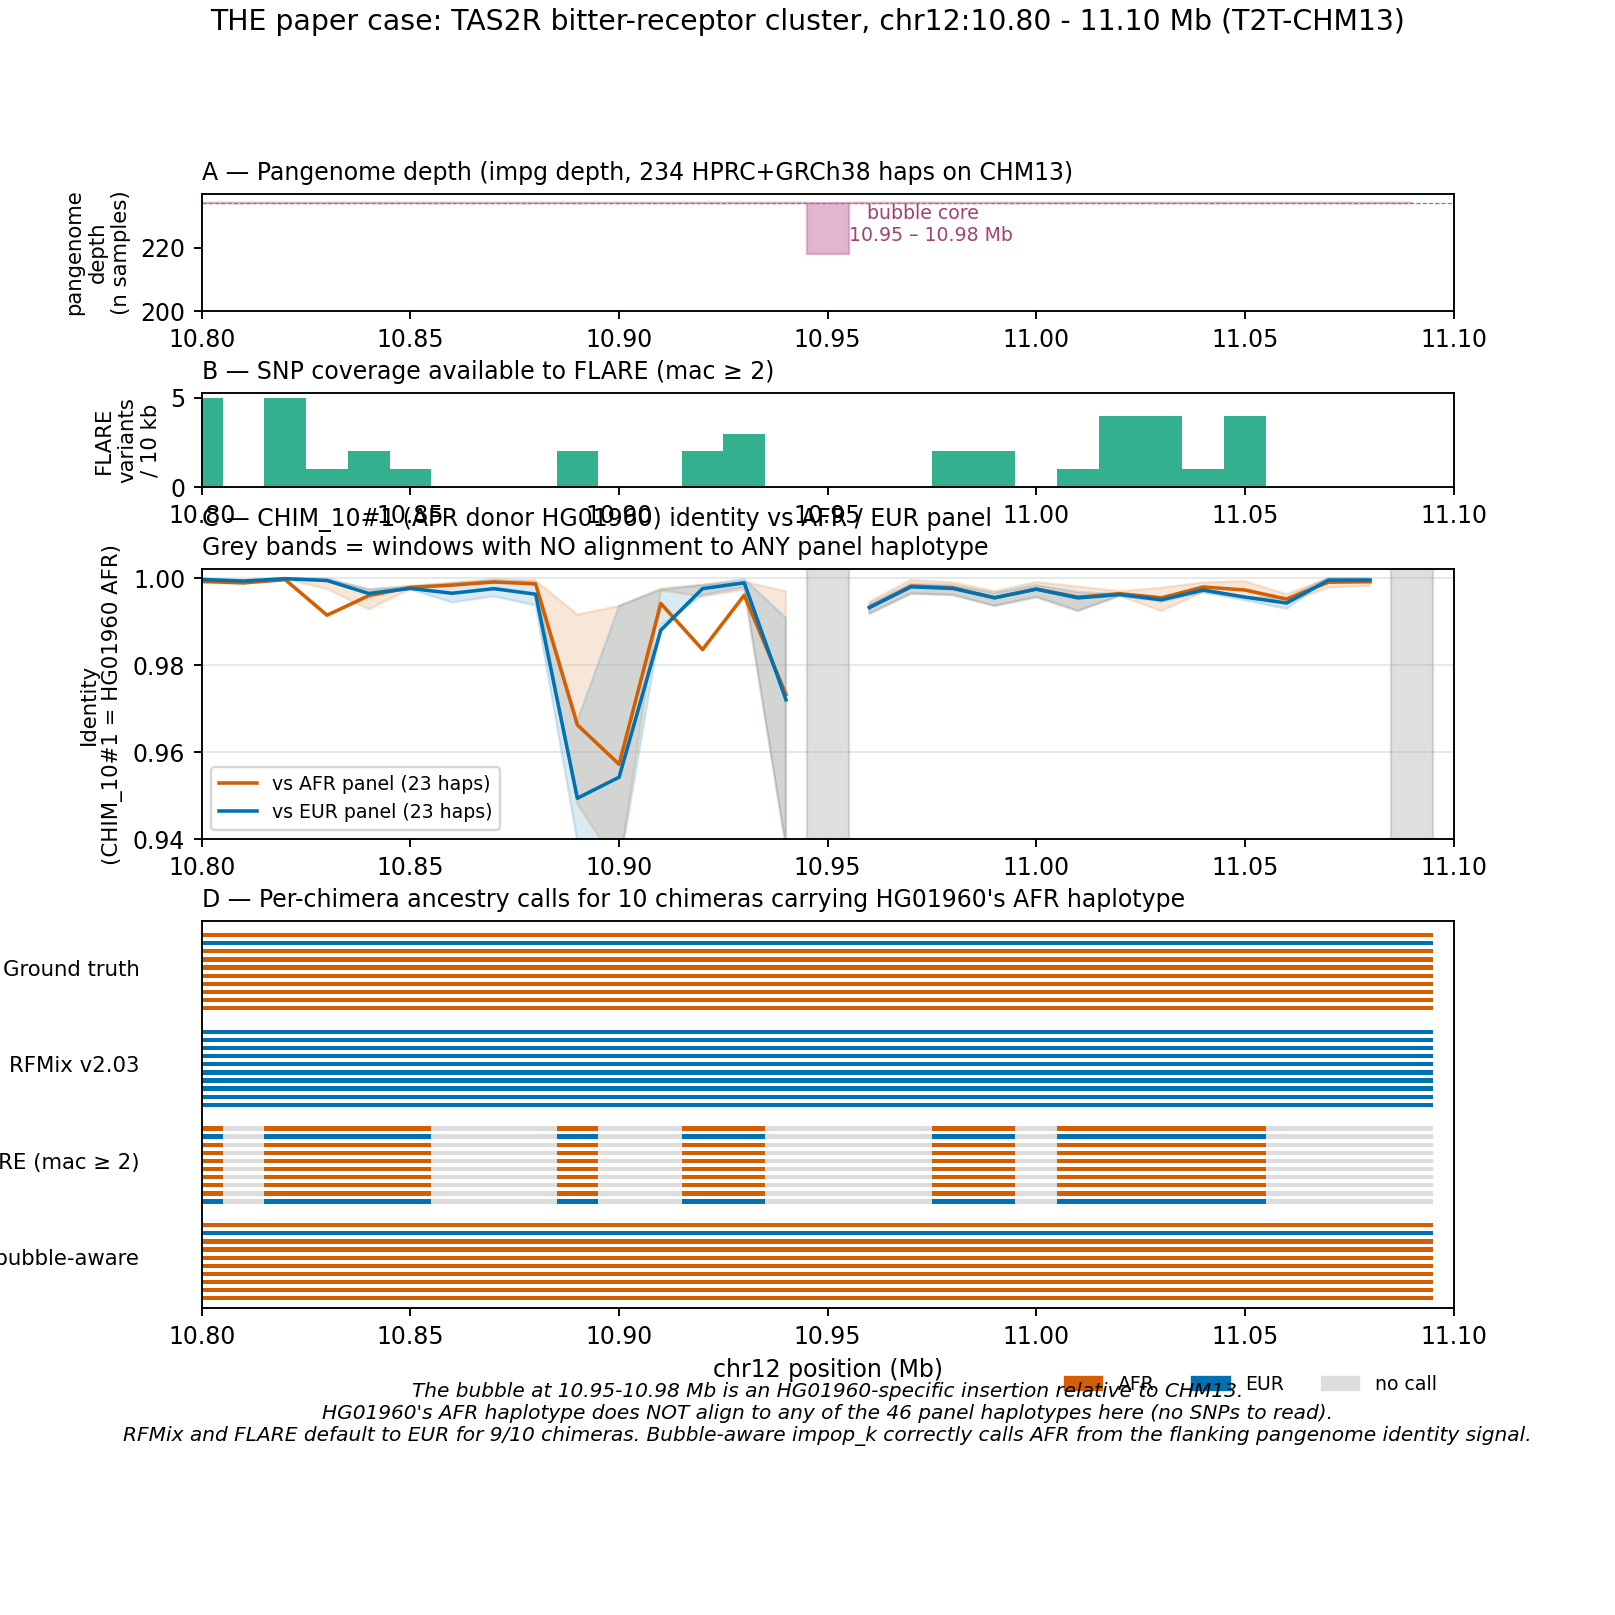
\includegraphics[width=0.5\textwidth]{fig_tas2r_bubble.png}
\caption{TAS2R structural haplotype at chr12:10.95--10.98\,Mb. \textbf{A)}~Pangenome depth from \texttt{impg depth} drops to 218/234 across the bubble; the 16 missing haplotypes are all African-enriched. \textbf{B)}~FLARE per-window SNP density collapses inside the bubble. \textbf{C)}~Query identity for HG01960-derived chimeras drops against the EUR panel and stays high against the AFR panel only inside the bubble. \textbf{D)}~Per-chimera ancestry calls for the 10 chimeras built from HG01960 as the AFR donor: bubble-aware \texttt{$impop_k$} matches the ground truth (9 AFR + 1 EUR); RFMix and FLARE call EUR for the 9 AFR-ground-truth chimeras.}
\label{fig:tas2r}
\end{figure}

\subsubsection{Cattle breeds}
\label{sec:cattle}

Here we assess a different question: when haplotype-resolved assemblies span species or subspecies, windowed identity can quantify which lineage each genomic region resembles most closely. We tested this on bovine chr1 (158\,Mb) from a publicly available super-pangenome~\cite{bovine_superpangenome} using the deposited assembly archive~\cite{bovine_superpangenome_data}. The panel includes four taurine breeds (Brown Swiss, Original Braunvieh, Highland, Piedmontese; \emph{Bos taurus taurus}), a single indicine breed (Nellore; \emph{Bos taurus indicus}), and an outgroup (Gaur, \emph{Bos gaurus}). A two-state model compares each query window against taurine (four breeds pooled) and indicine (Nellore alone), assigning it to the more similar group. Taurine and indicine cattle diverged 250,000 to 500,000 years ago~\cite{chen2019bos}.

Mean pairwise identity is 0.996 within taurine, 0.989 for taurine--indicine, and 0.979 for taurine--Gaur (Fig.~\ref{fig:cattle}A). As a control, the two-state model assigns $>$99.8\% of windows to taurine for both Original Braunvieh and Piedmontese. For Gaur, whose lineage predates the taurine--indicine split~\cite{chen2019bos}, the comparison instead asks which lineage each window resembles more closely. Across three chromosomes, 76\% of Gaur windows show higher identity to taurine and 24\% to indicine (Fig.~\ref{fig:cattle}C,D), largely reflecting incomplete lineage sorting at the three-taxon divergence. A slight excess similarity to Nellore (identity difference of 0.001) may reflect post-speciation gene flow~\cite{mei2023indicine}, though a larger panel would be needed to distinguish introgression from ILS.

A UPGMA tree from pairwise divergence ($1 - \text{identity}$) recovers the expected  phylogeny~\cite{chen2019bos}: taurine breeds form a monophyletic clade, Nellore branches next, and Gaur roots the tree (Fig.~\ref{fig:cattle}B). Branch lengths reflect increasing divergence: $d \approx 0.004$ within taurine, $\approx 0.011$ to indicine, and $\approx 0.021$ to Gaur. This topology matches the established \emph{Bos} species tree.

\begin{figure*}[t]
\centering
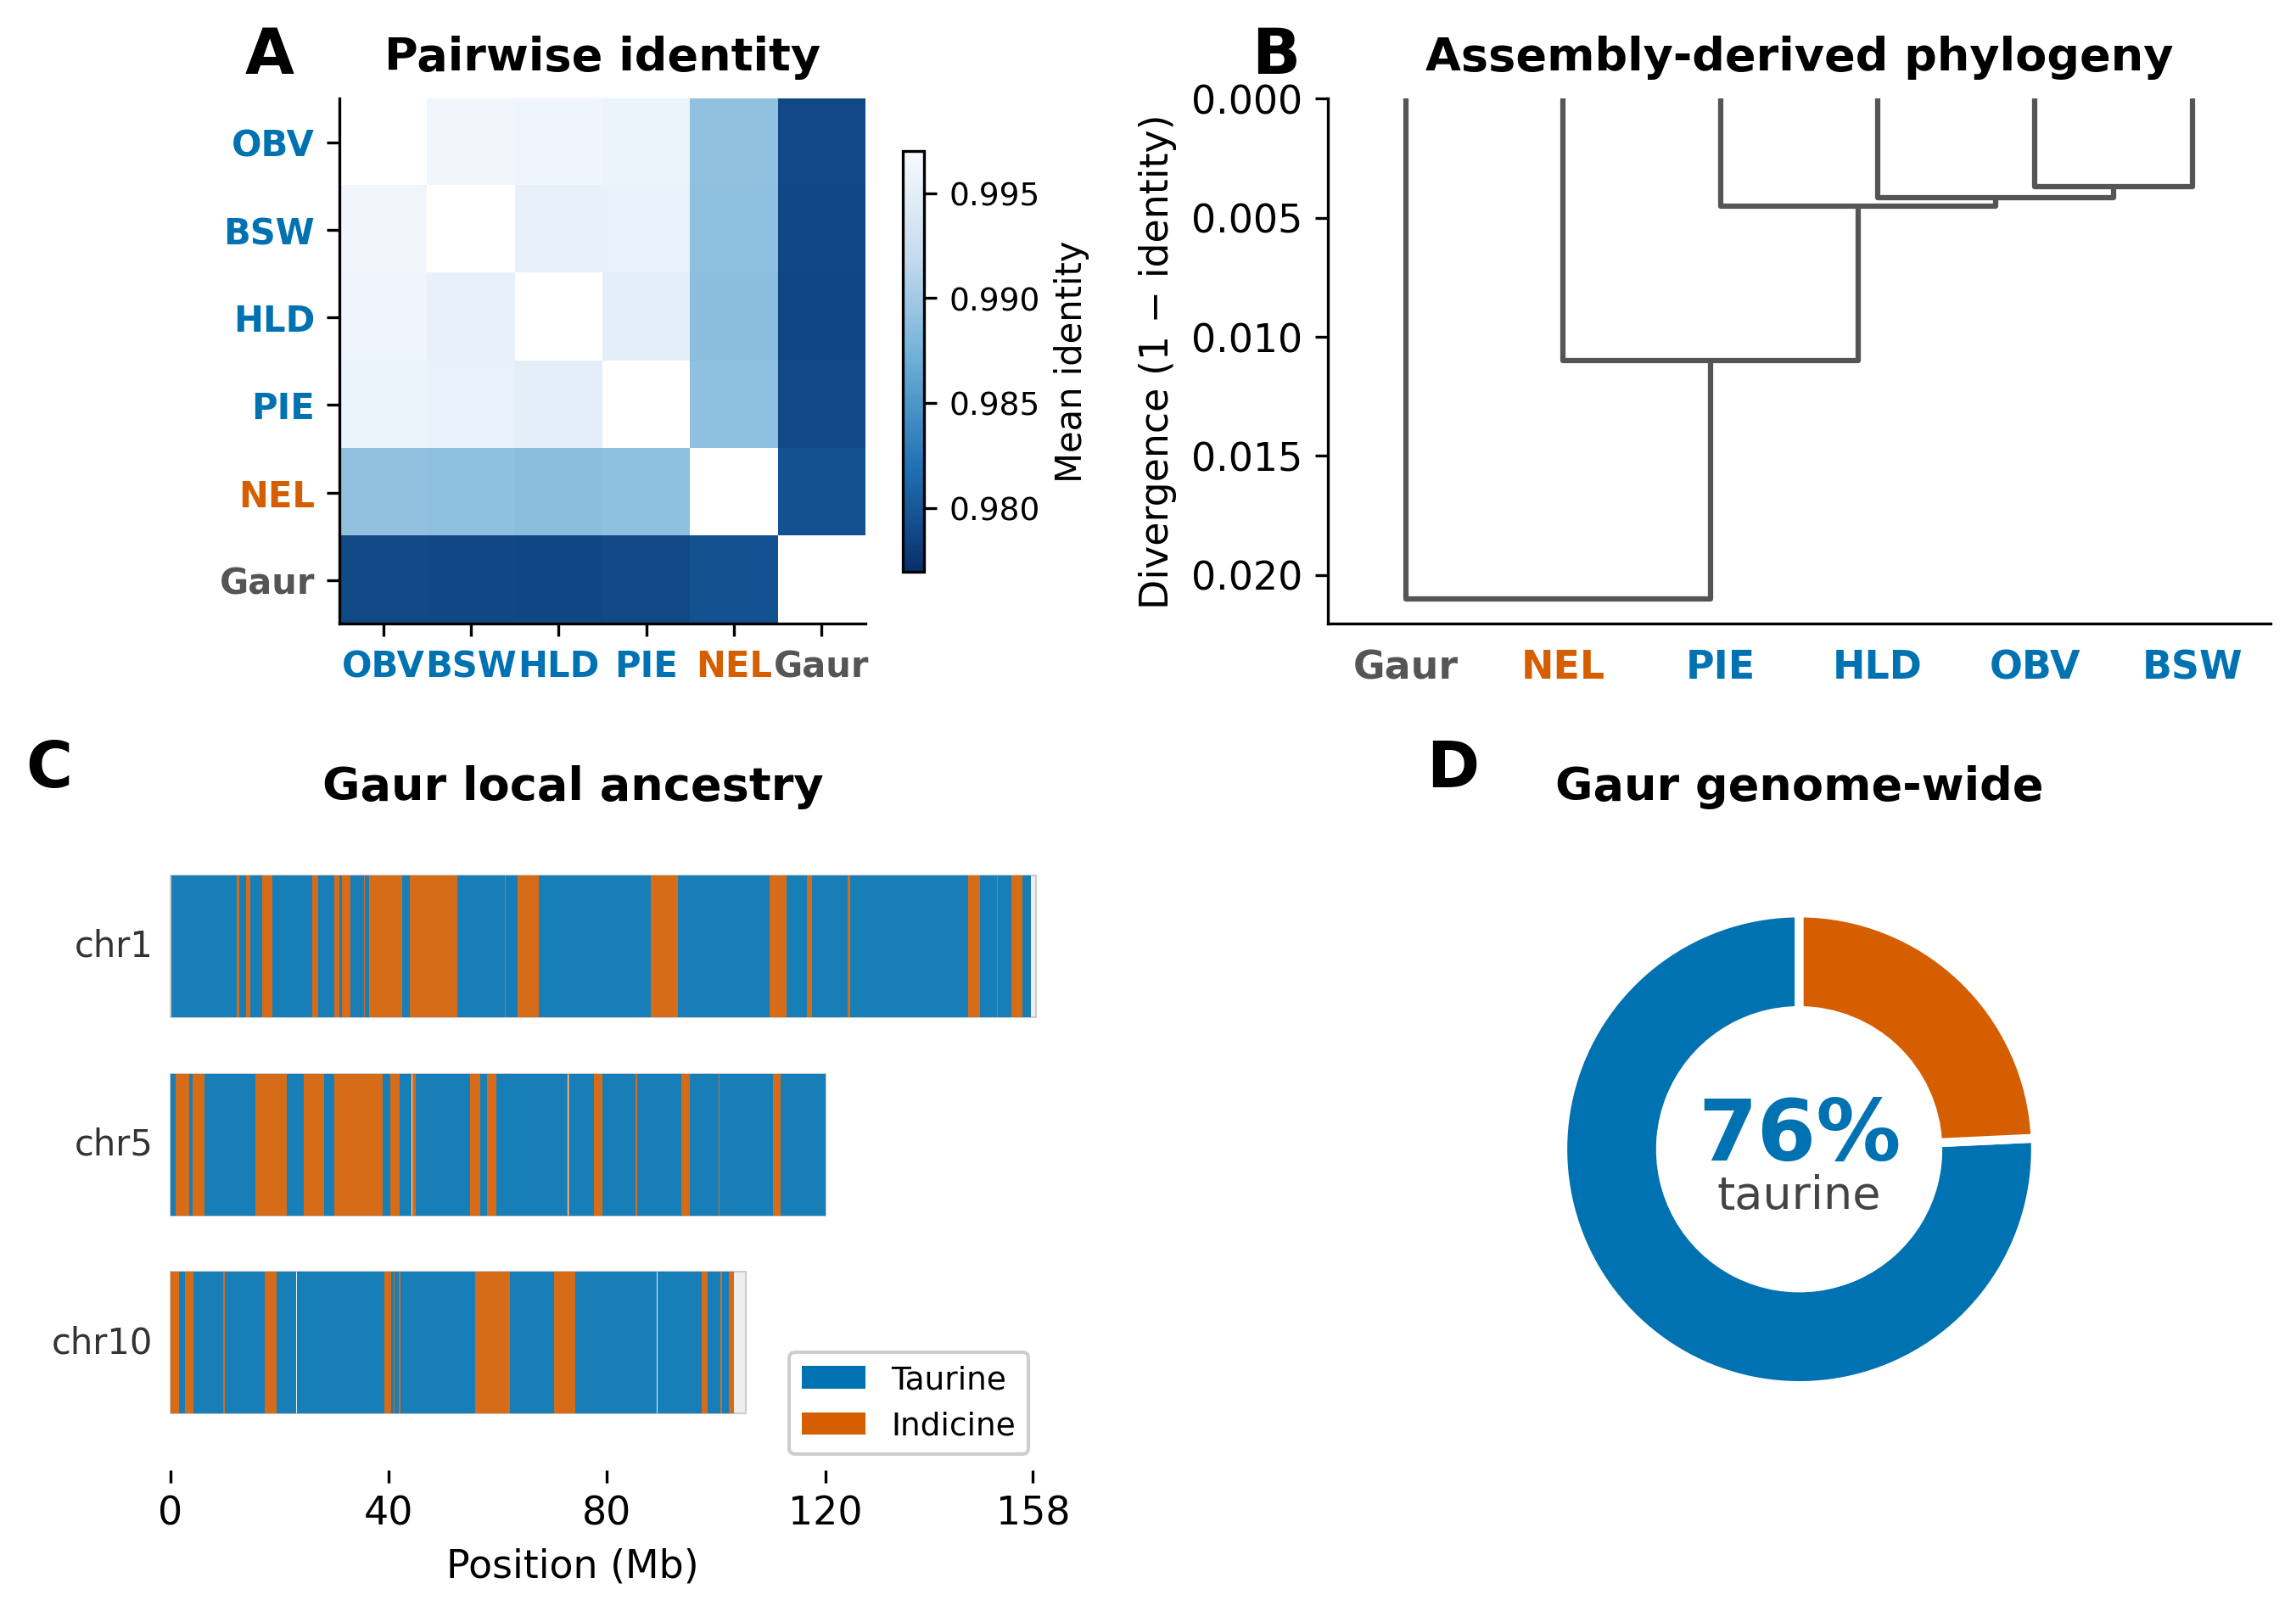
\includegraphics[width=0.80\textwidth]{fig5_cattle.png}
\caption{Bovine subspecies structure (chr1, 158\,Mb). \textbf{A)}~Pairwise identity heatmap. \textbf{B)}~UPGMA phylogeny from assembly-derived divergence. \textbf{C)}~Gaur per-window similarity assignment (taurine vs.\ indicine) across three chromosomes. \textbf{D)}~Genome-wide proportion (76\% taurine-like).}
\label{fig:cattle}
\end{figure*}

\subsubsection{Founder haplotype mapping in BXD recombinant inbred mice}
\label{sec:bxd}

The BXD panel is a set of recombinant inbred mouse lines derived from C57BL/6J (B6) and DBA/2J (D2). After repeated generations of sibling mating, each line is nearly homozygous, and its genome is a mosaic of the two founder haplotypes (Fig.~\ref{fig:bxd}A). Because the two founders are known, the problem reduces to a two-state ancestry assignment at each locus: B6 or D2. We computed windowed pairwise identity (10\,kb windows via \texttt{impg}) between each of 10 BXD offspring assemblies and both founder genomes on mouse Chr01 (207\,Mb), then assigned each window to the founder with higher identity.

The resulting profiles (Fig.~\ref{fig:bxd}B) show the expected mosaic structure: each line alternates between regions of B6 and D2 ancestry, with sharp transitions at recombination breakpoints. The proportion of B6 ancestry varies across lines (46--88\% on Chr01), and the breakpoint positions differ between individuals, consistent with independent meiotic histories. Regions where multiple lines share the same founder identity may reflect selection or low recombination. A systematic comparison with published BXD genotype maps is left for future work.

\begin{figure*}[t]
\centering
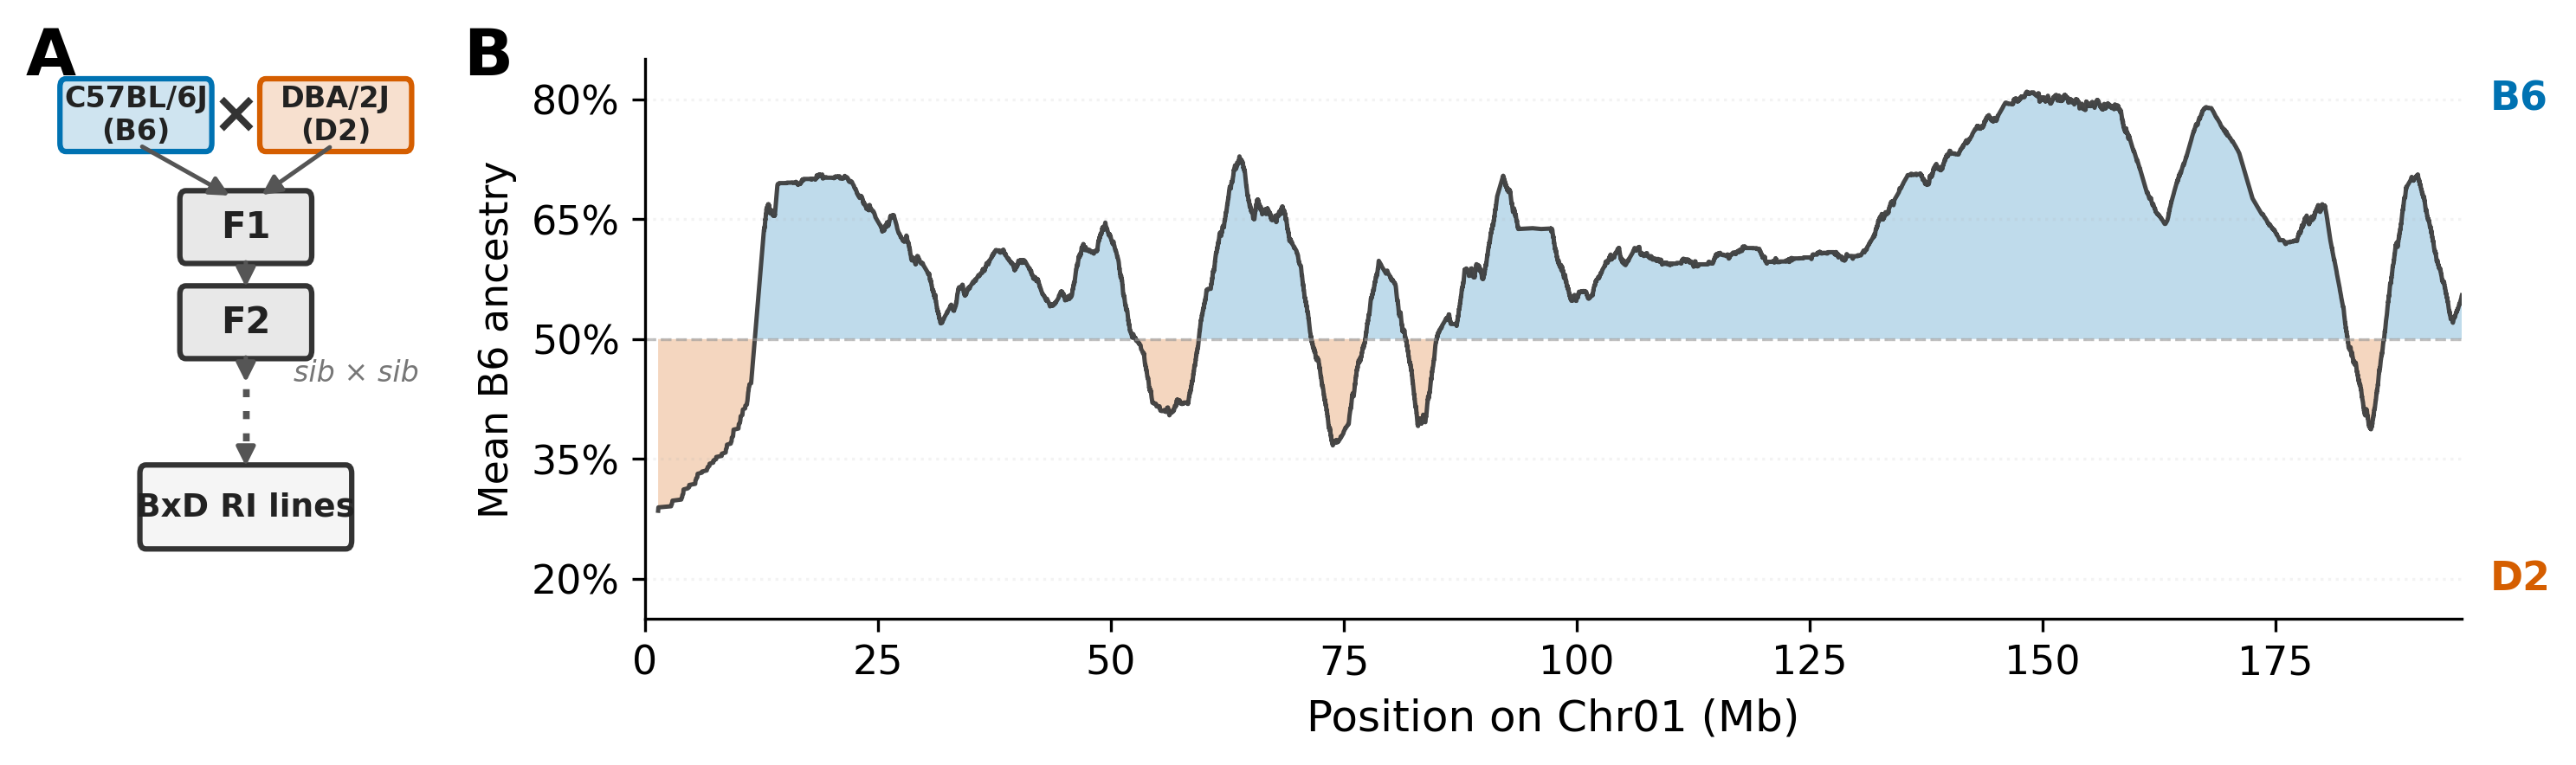
\includegraphics[width=0.95\textwidth]{fig6_bxd.png}
\caption{BXD mouse founder mapping (Chr01, 207\,Mb). \textbf{A)}~Inbreeding scheme: C57BL/6J (B6) $\times$ DBA/2J (D2) cross followed by sibling mating to produce RI lines. \textbf{B)}~Mean B6 ancestry across 10 lines, smoothed in 2\,Mb windows. Transitions mark recombination breakpoints.}
\label{fig:bxd}
\end{figure*}

% ──────────────────────────────────────────────────────────────
\section{Discussion}

The identity contrasts in 10\,kb pangenome windows are small ($\Delta \approx 0.001$ to $0.003$), but consistent across windows, and HMMs can integrate them into contiguous tracts. The results above suggest this works across several settings: simulated and real human data, a three-generation pedigree, and a cross-species bovine panel. The same code ran on all of them because the input is pairwise identity, not a species-specific variant set.

There are clear limitations. IBD boundary precision is constrained by the 10\,kb window. Identity is computed relative to a single reference genome, so regions with structural variation or poor alignment can drop out. Pairwise computation scales quadratically with the number of haplotypes, limiting direct application to large cohorts.

The practical ceiling is the identity gap between populations. For closely related groups ($\Delta \approx 0.001$), the signal is barely above noise, and larger reference panels are needed. The upcoming HPRC Release~3 ($>$350 individuals) should help. The HMM runs in seconds per chromosome; the bottleneck is the identity computation via \texttt{impg}. The relationship between local coalescence time and sequence identity also underlies PSMC~\cite{li2011psmc}, which infers demographic history from heterozygosity along a single diploid genome. Our approach exploits the same relationship but targets IBD status and ancestry at each locus, using continuous identity from pangenome alignments rather than binary heterozygosity. As assembly costs continue to fall and pangenome reference panels grow, the identity signal available to these models will only improve.

\bibliographystyle{unsrtnat}
\bibliography{references}

% ──────────────────────────────────────────────────────────────
\section*{Data availability}
HPRC assemblies and alignments~\cite{liao2023hprc} are available through the HPRC data portal. CEPH~1463 assemblies are available from the Platinum Pedigree Consortium S3 bucket (\texttt{s3://platinum-pedigree-data/assemblies/}); inheritance vectors from the Platinum-Pedigree-Inheritance repository~\cite{platinum_ped}. Bovine assemblies from Zenodo~\cite{bovine_superpangenome_data}. All derived data and figure-generation scripts are in the code repository.

\section*{Code availability}
\texttt{$impop_k$} and step-by-step tutorials are available at \url{https://github.com/MarsicoFL/impopk}.

\end{document}
